% Experiment 4 — full scientific submission package
\documentclass[11pt,a4paper]{article}

\usepackage[margin=2.5cm]{geometry}
\usepackage{graphicx}
\usepackage{booktabs}
\usepackage{amsmath}
\usepackage{xurl}
\usepackage{hyperref}
\usepackage{parskip}
\usepackage{enumitem}
\usepackage{fvextra}
\usepackage[most]{tcolorbox}

\newcommand{\studentname}{Mahmudul Hasan}
\newcommand{\studentid}{4125999049}
\newcommand{\reportdate}{May 23, 2026}

\makeatletter
\g@addto@macro\UrlBreaks{\do\ }
\makeatother

\newcommand{\LabCodeRoot}{files}

\newcommand{\filebox}[2]{%
\begin{tcolorbox}[
  enhanced,
  colback=gray!6,
  colframe=black!55,
  title={#1},
  fonttitle=\bfseries\ttfamily\footnotesize,
  arc=1.5mm,
  boxrule=0.7pt,
  breakable,
  width=\linewidth,
  before skip=0.8em,
  after skip=0.8em,
]
\VerbatimInput[fontsize=\footnotesize,breaklines=true,breakanywhere=true]{\LabCodeRoot/#2}
\end{tcolorbox}%
}

\title{Experiment Report: Specialized Experiment 4\\Flood Inundation Analysis (DEM-based)}
\author{\studentname \quad (Student ID: \studentid)}
\date{\reportdate}

\begin{document}
\maketitle

\begin{abstract}
Bathtub inundation on a reproducible 100$\times$100 synthetic DEM: mask $z<h$, depth $\max(0,h-z)$, area and volume statistics, GIS-style maps with elevation contours, annotated growth on the flood curve, seed sensitivity, and performance benchmarks. All guide deliverables are present; extensions remain assignment-safe (no routing or PDE solvers).
\end{abstract}

\begin{tcolorbox}[
  colback=blue!4,
  colframe=blue!55!black,
  title=\textbf{Key Findings (Executive Summary)},
  fonttitle=\bfseries,
  arc=2mm,
]
\begin{tabular}{@{}ll@{}}
\textbf{Finding} & \textbf{Result} \\
\hline
DEM range (seed 42) & 36.0--68.8~m \\
Flooded @ 40~m / 50~m & 2.41\% / 25.25\% \\
Flood volume @ 40~m / 50~m & $\approx$285 / $\approx$12{,}278~m$^3$ \\
Curve resolution & 0.5~m steps, 21 points, monotonic \\
Seed sensitivity @ 50~m & 25.25\% / 25.45\% / 25.04\% (seeds 42/7/99) \\
Validation checklist & 9/9 PASS \\
Automated tests & 21 passed \\
\end{tabular}
\end{tcolorbox}

\section{Role in the Integrated Smart Water Pipeline}
Experiment~4 is the \textbf{impact assessment stage} at the end of the pipeline. Given a water-surface elevation (design flood stage or reservoir spill level), it:
\begin{itemize}[noitemsep]
  \item maps inundation extent, depth, flooded area percentage, and stored flood volume on a reproducible synthetic DEM;
  \item documents monotonic stage--area--volume behaviour for defensible emergency-response interpretation;
  \item supports decisions triggered by upstream alerts (Experiment~1), runoff forcing (Experiment~2), and release scenarios (Experiment~3).
\end{itemize}
It translates hydrologic and operational inputs into spatial flood consequences for planning and communication.

%=============================================================================
\section{Part 1: DEM Data Preparation (15\%)}
%=============================================================================

\subsection{Synthetic terrain}
Grid: 100$\times$100, \texttt{rng(42)}, central valley + hills + ridge + noise, clipped 30--80~m. Cell size 1~m. \texttt{dem\_data.npy} saved by \texttt{load\_dem()}.

\begin{figure}[htbp]
  \centering
  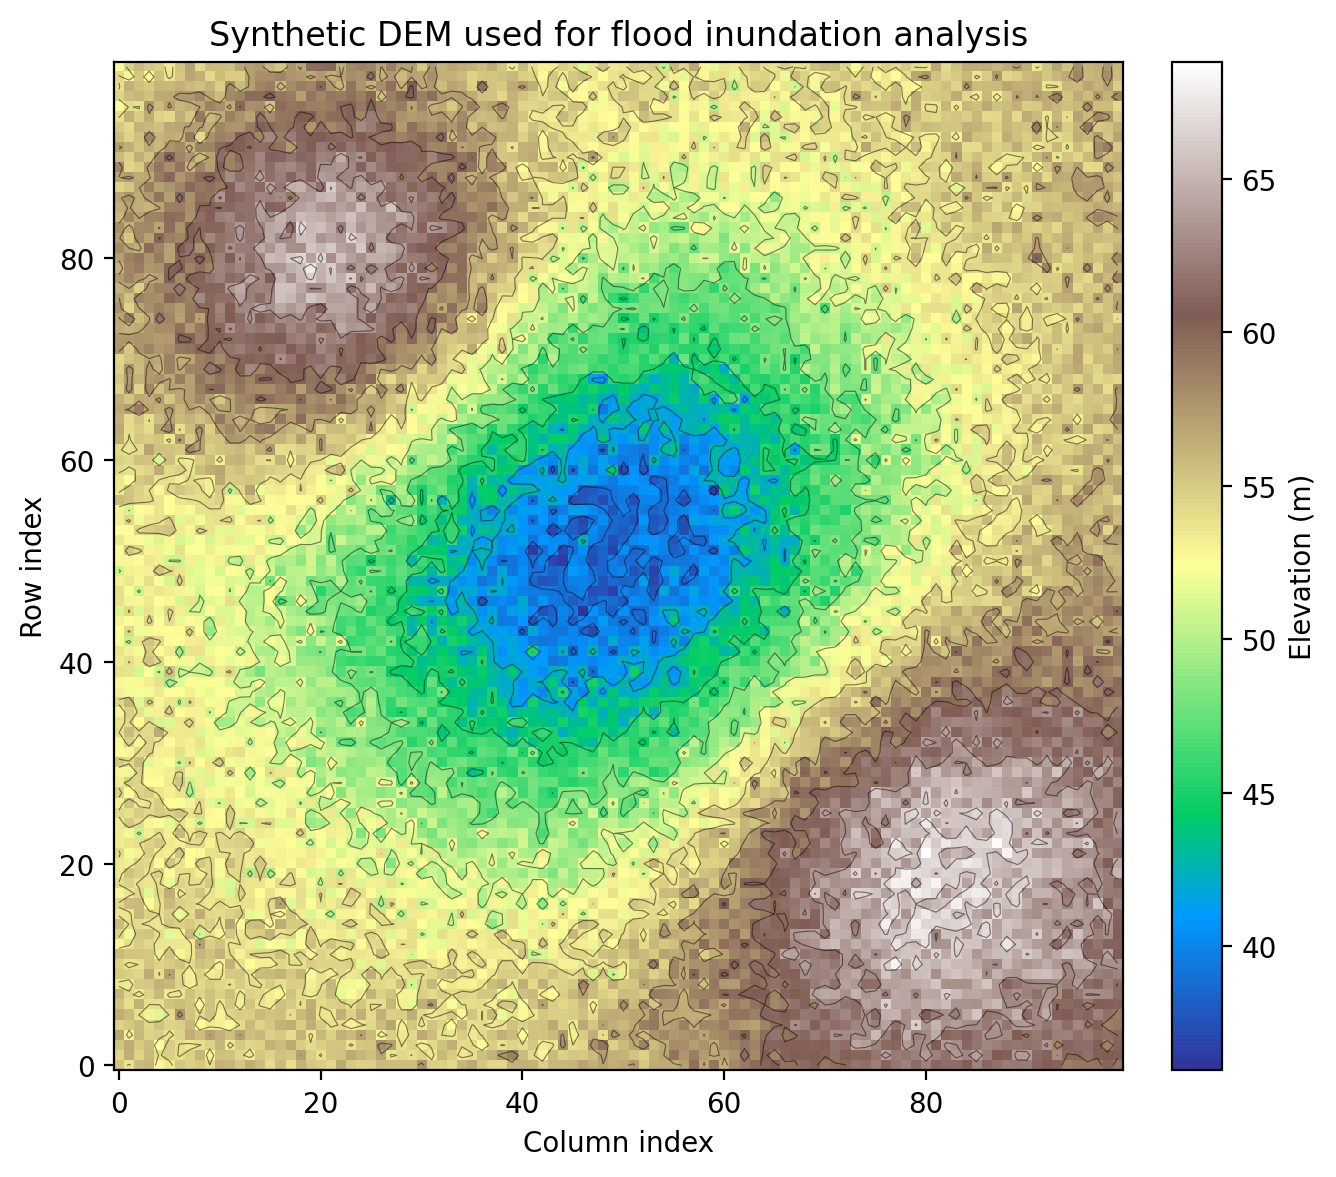
\includegraphics[width=0.78\linewidth,keepaspectratio]{screenshots/dem_overview.png}
  \caption{Synthetic DEM with terrain colormap and elevation contours.}
  \label{fig:dem}
\end{figure}

\begin{figure}[htbp]
  \centering
  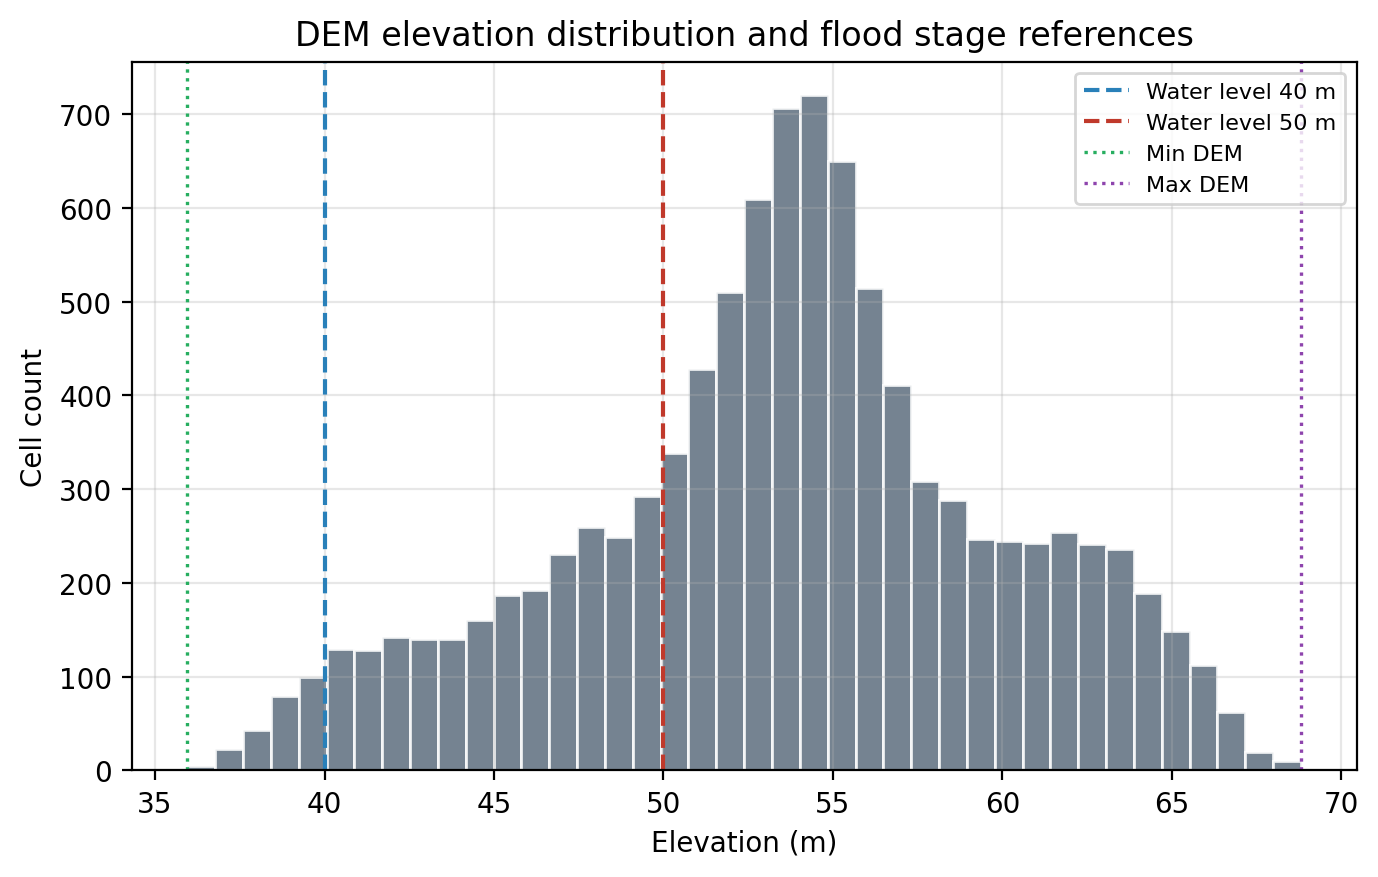
\includegraphics[width=0.78\linewidth,keepaspectratio]{screenshots/dem_histogram.png}
  \caption{Elevation histogram: vertical lines at 40~m and 50~m stage explain rapid inundation growth once $h$ crosses dense elevation bins.}
  \label{fig:hist}
\end{figure}

\begin{figure}[htbp]
  \centering
  
\includegraphics[width=0.72\linewidth,keepaspectratio]{screenshots/architecture.png}
  \caption{Pipeline: DEM $\rightarrow$ \texttt{calculate\_flood} $\rightarrow$ visualization $\rightarrow$ validation.}
  \label{fig:arch}
\end{figure}

%=============================================================================
\section{Part 2: Flood Calculation (25\%)}
%=============================================================================

\textbf{Mask:} $z_{ij}<h$. \textbf{Depth:} $\max(0,h-z)$ on wet cells. \textbf{Volume:} $V=\sum d_{ij} A_{\mathrm{cell}}$.

\begin{table}[htbp]
  \centering
  \caption{Statistics at required levels (seed 42 DEM).}
  \label{tab:levels}
  \begin{tabular}{@{}rrrr@{}}
    \toprule
    $h$ (m) & Flooded (\%) & Mean depth wet (m) & Volume (m$^3$) \\
    \midrule
    40 & 2.41 & 1.18 & $\approx$285 \\
    45 & 10.92 & --- & --- \\
    50 & 25.25 & 4.86 & $\approx$12{,}278 \\
    \bottomrule
  \end{tabular}
\end{table}

%=============================================================================
\section{Part 3: Visualization (25\%)}
%=============================================================================

Maps: grayscale DEM + black elevation contours + blue depth overlay (\texttt{origin='lower'}, 300~DPI). Required: \texttt{flood\_extent\_40m.png}, \texttt{flood\_extent\_50m.png}.

\begin{figure}[htbp]
  \centering
  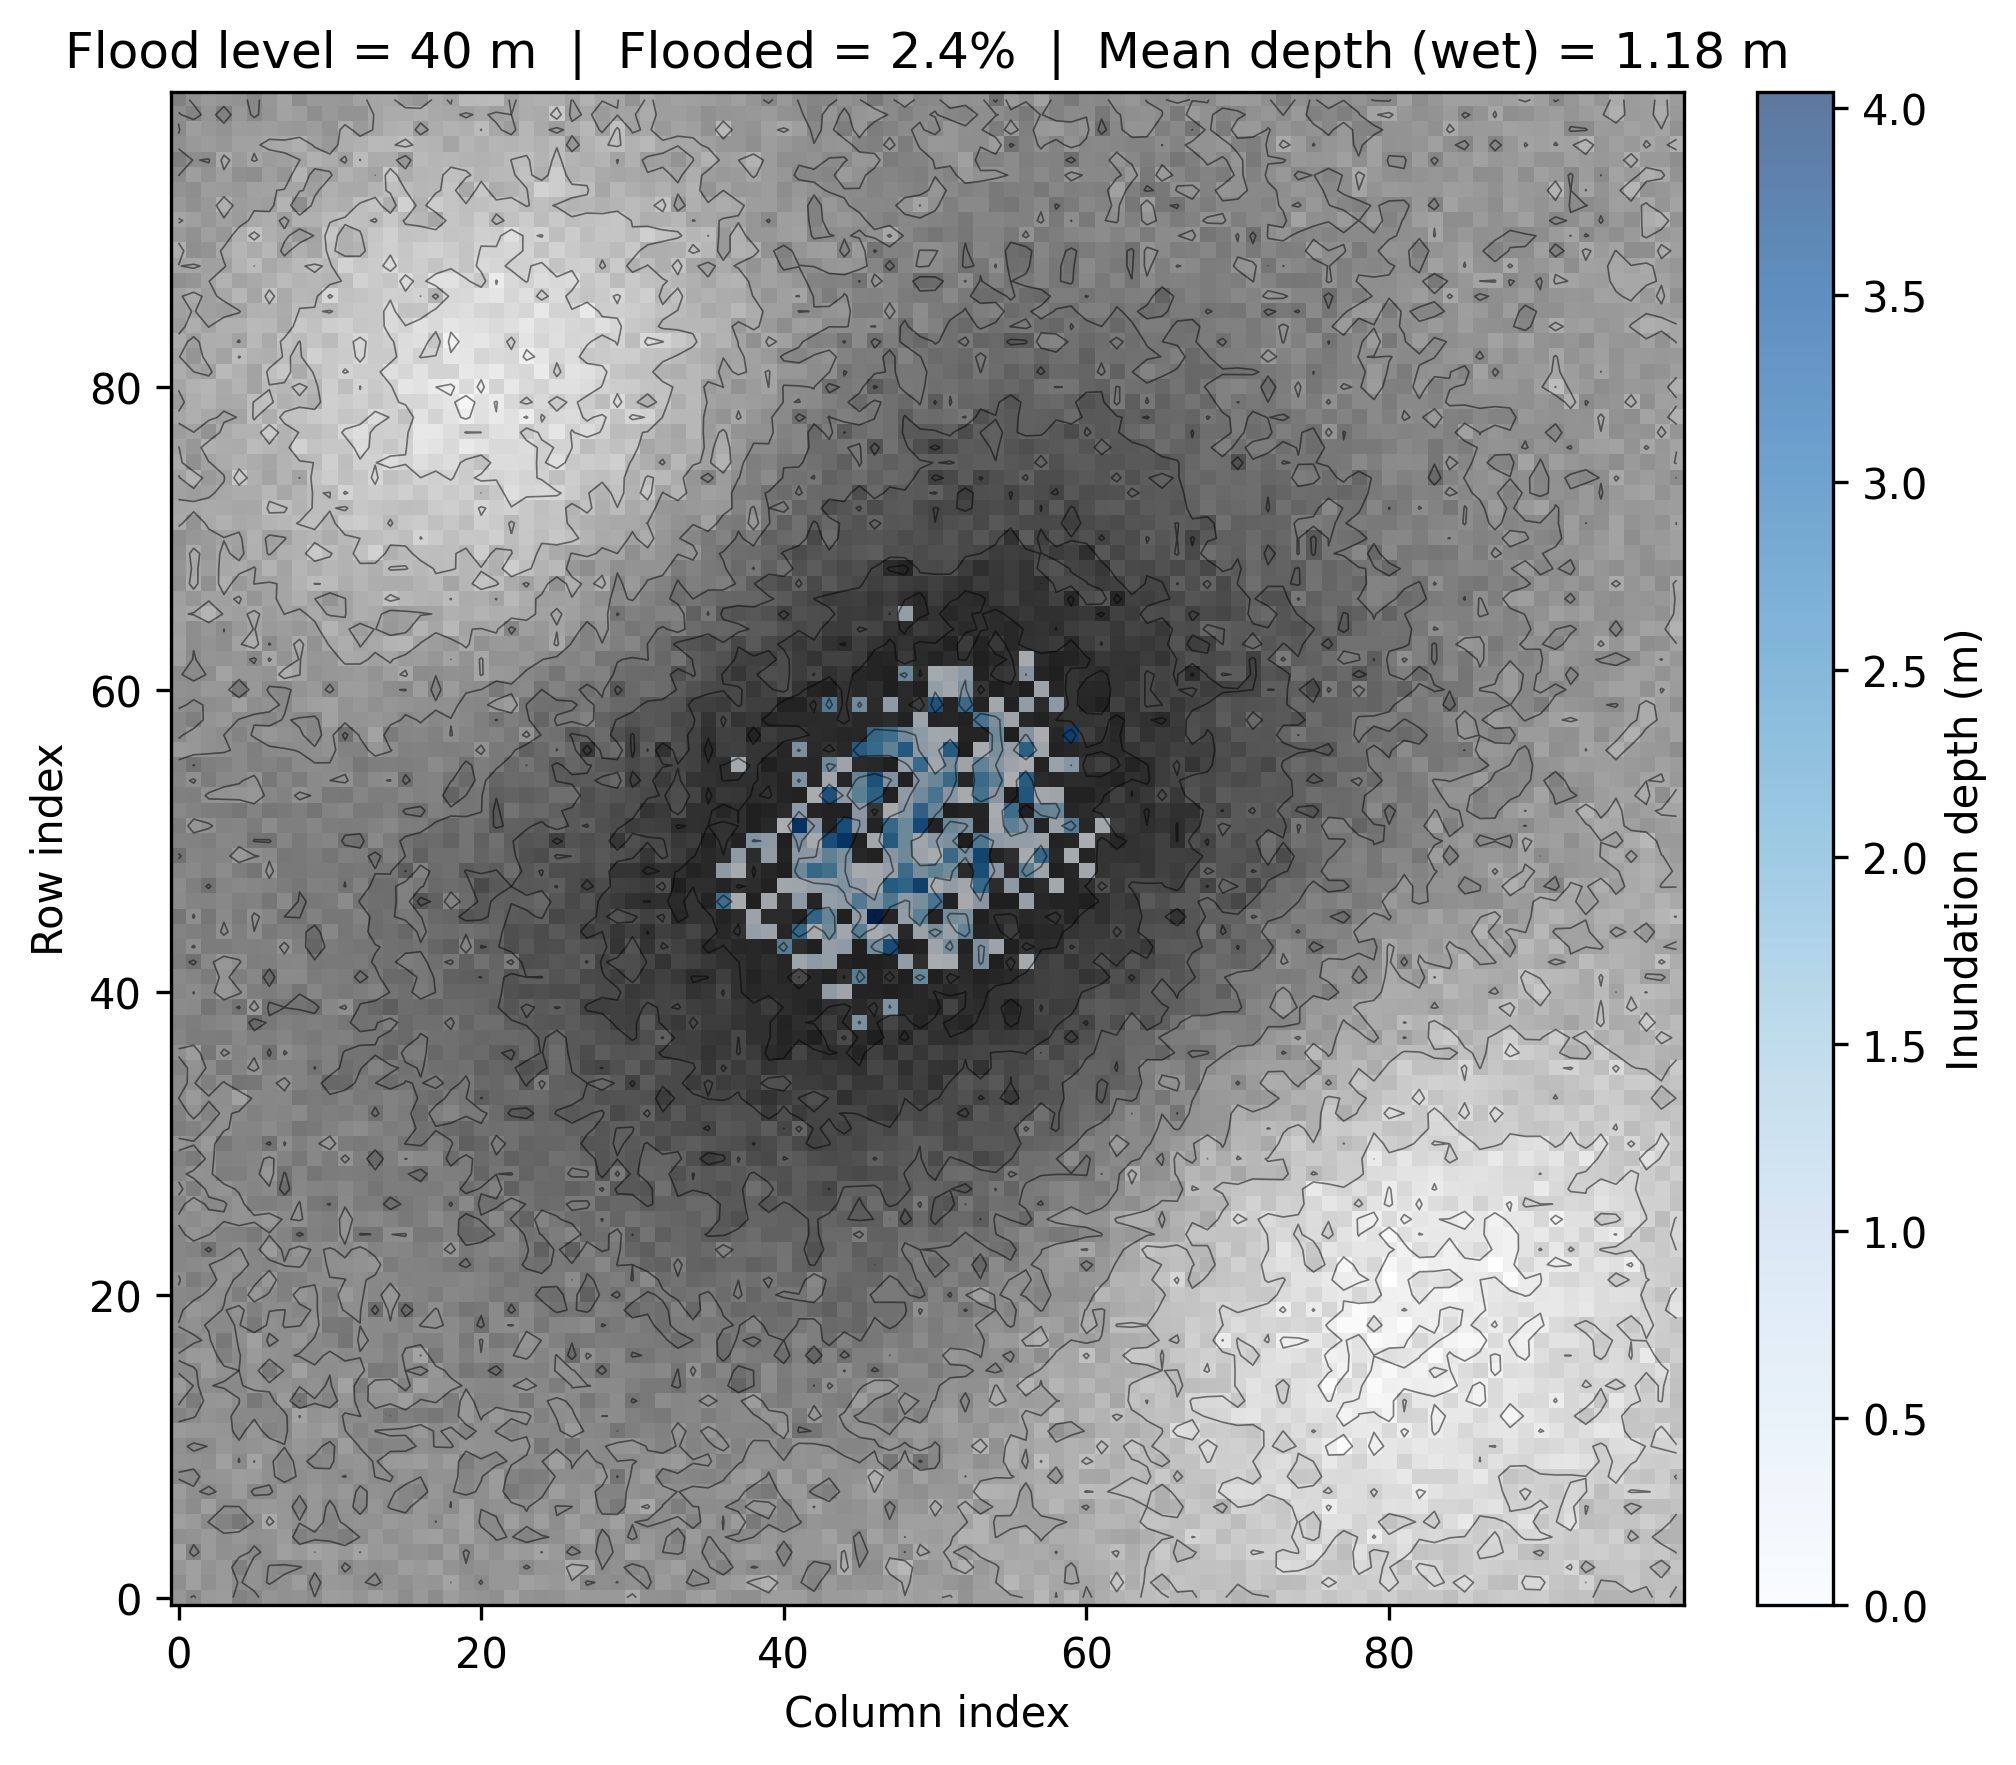
\includegraphics[width=\linewidth]{screenshots/flood_extent_40m.png}
  \caption{40~m stage: valley cells first (2.41\% flooded).}
  \label{fig:extent40}
\end{figure}

\begin{figure}[htbp]
  \centering
  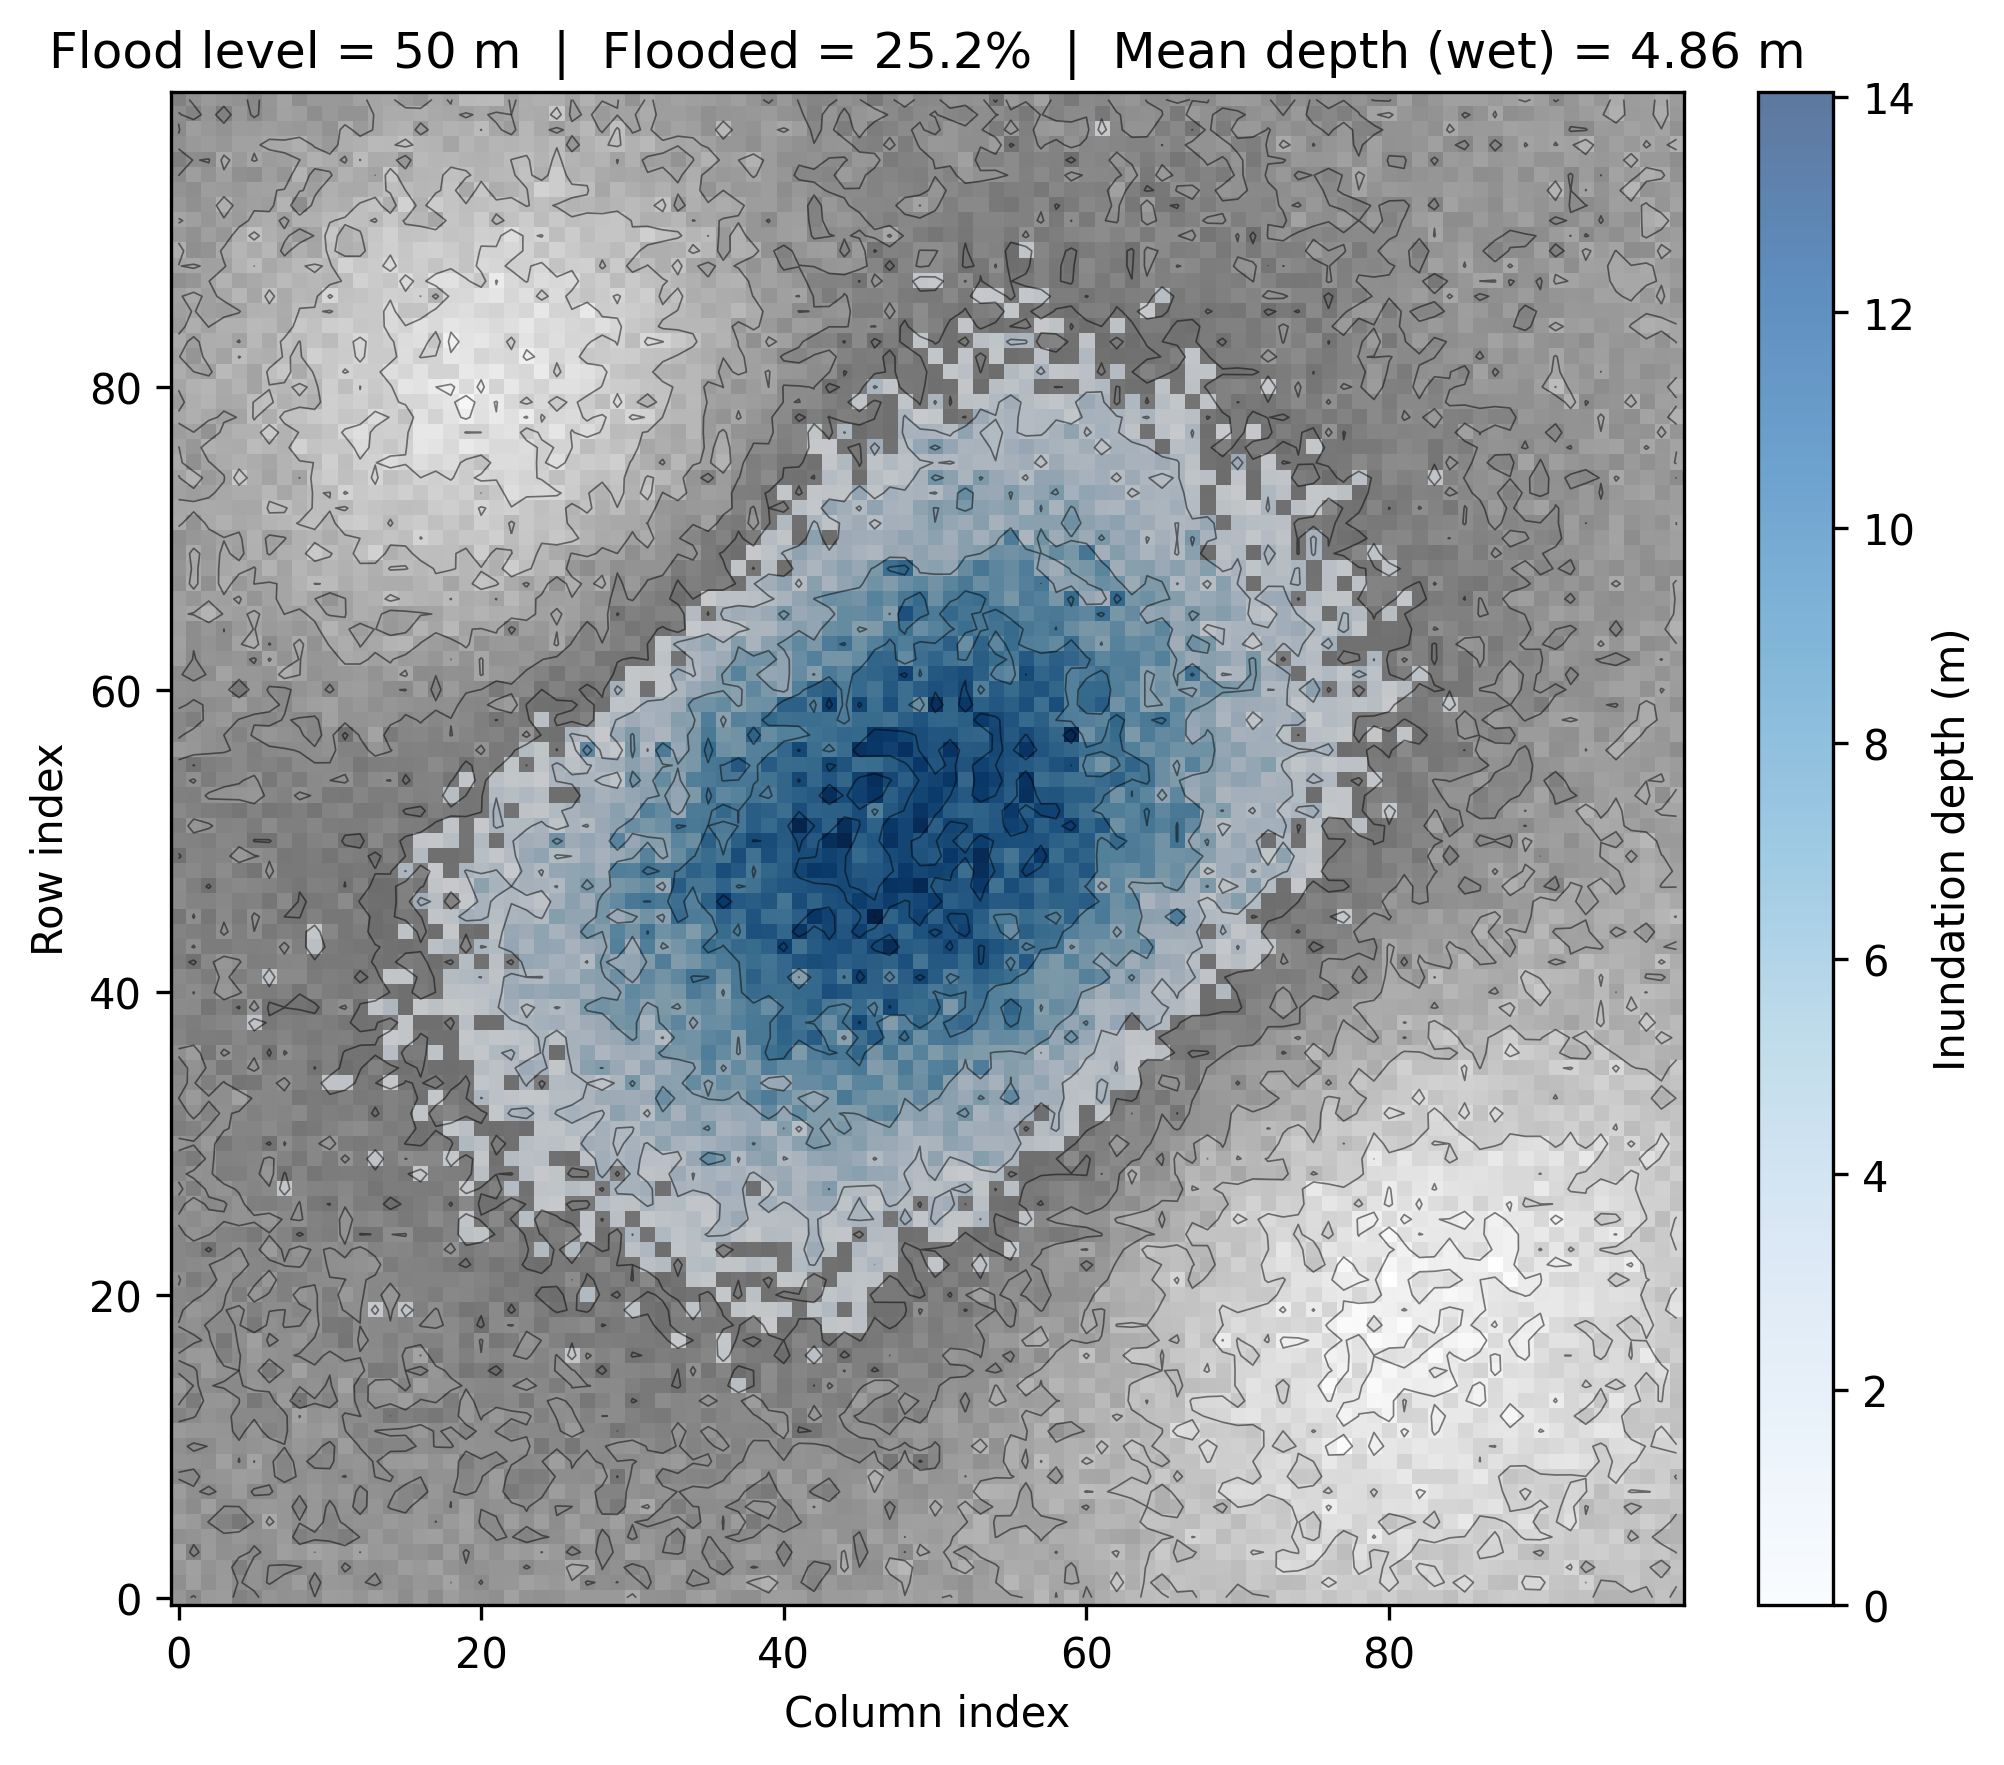
\includegraphics[width=\linewidth]{screenshots/flood_extent_50m.png}
  \caption{50~m stage: expanded connected inundation (25.25\%).}
  \label{fig:extent50}
\end{figure}

\begin{figure}[htbp]
  \centering
  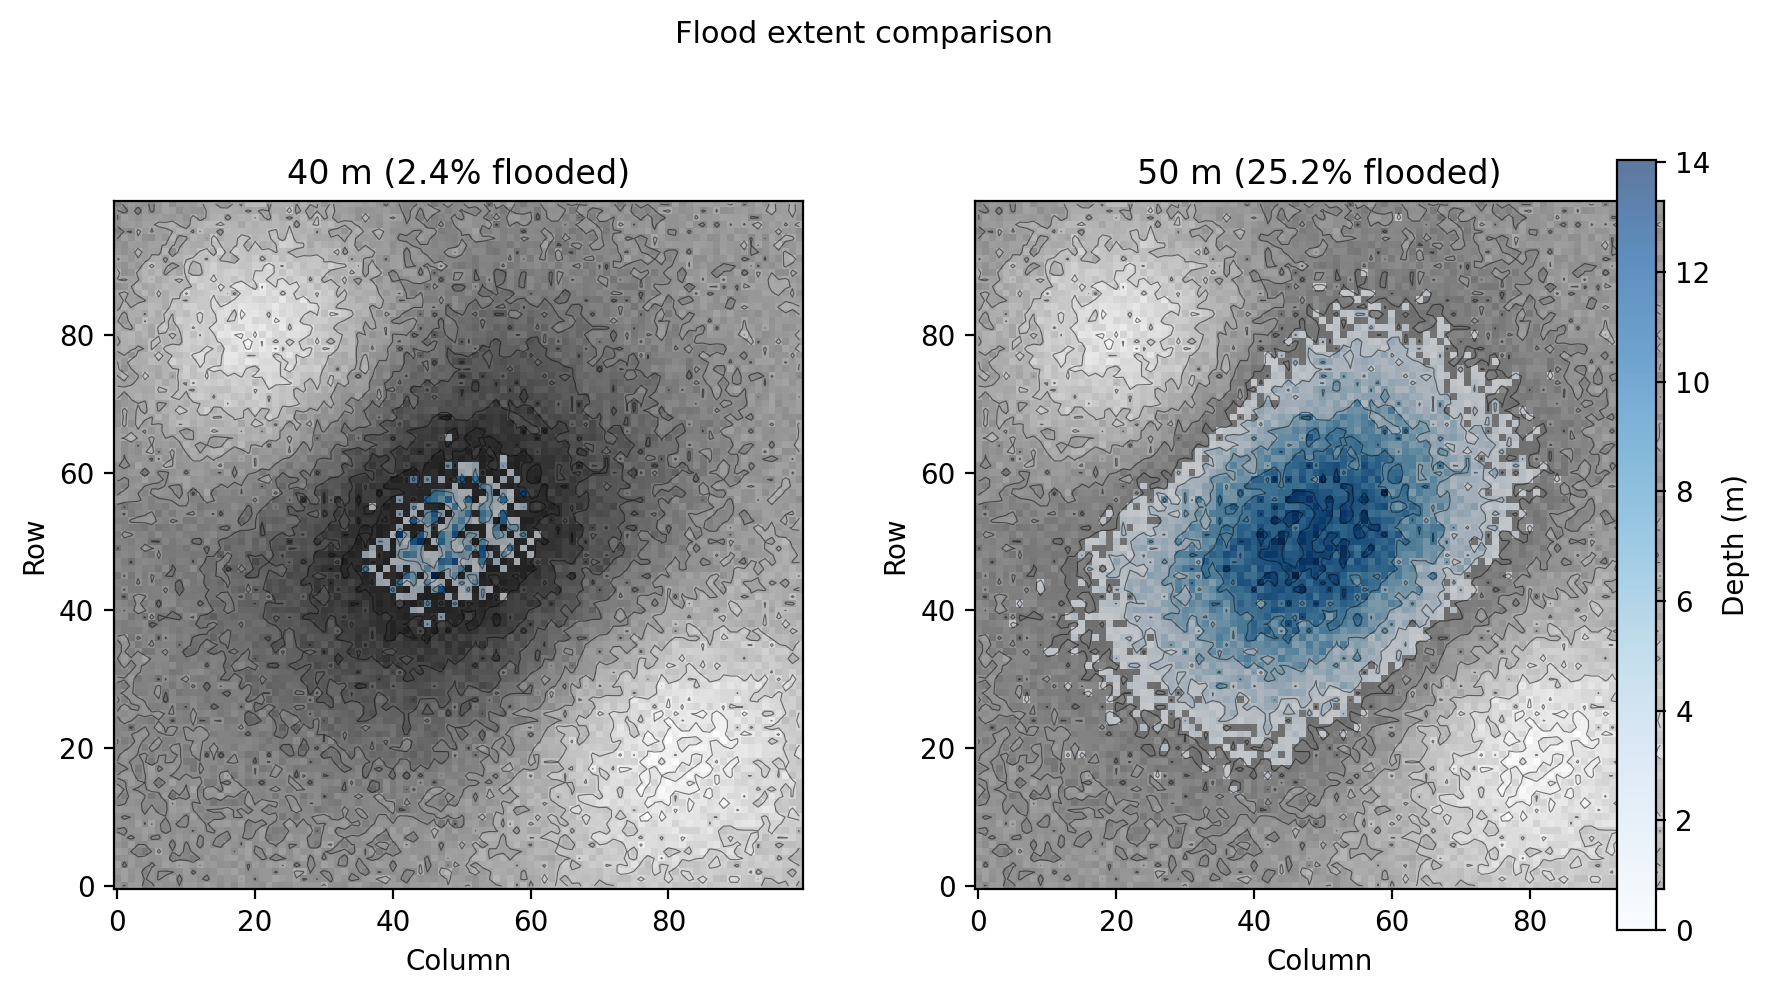
\includegraphics[width=\linewidth]{screenshots/flood_comparison_40_50m.png}
  \caption{Side-by-side comparison with contours.}
  \label{fig:compare}
\end{figure}

%=============================================================================
\section{Part 4: Dynamic Simulation (20\%)}
%=============================================================================

\texttt{simulate\_rising\_water()}: 40--50~m, step 0.5~m. \texttt{flood\_curve.png} annotates first flooding, 10\% threshold, and steepest growth segment; min/max DEM lines included.

\begin{figure}[htbp]
  \centering
  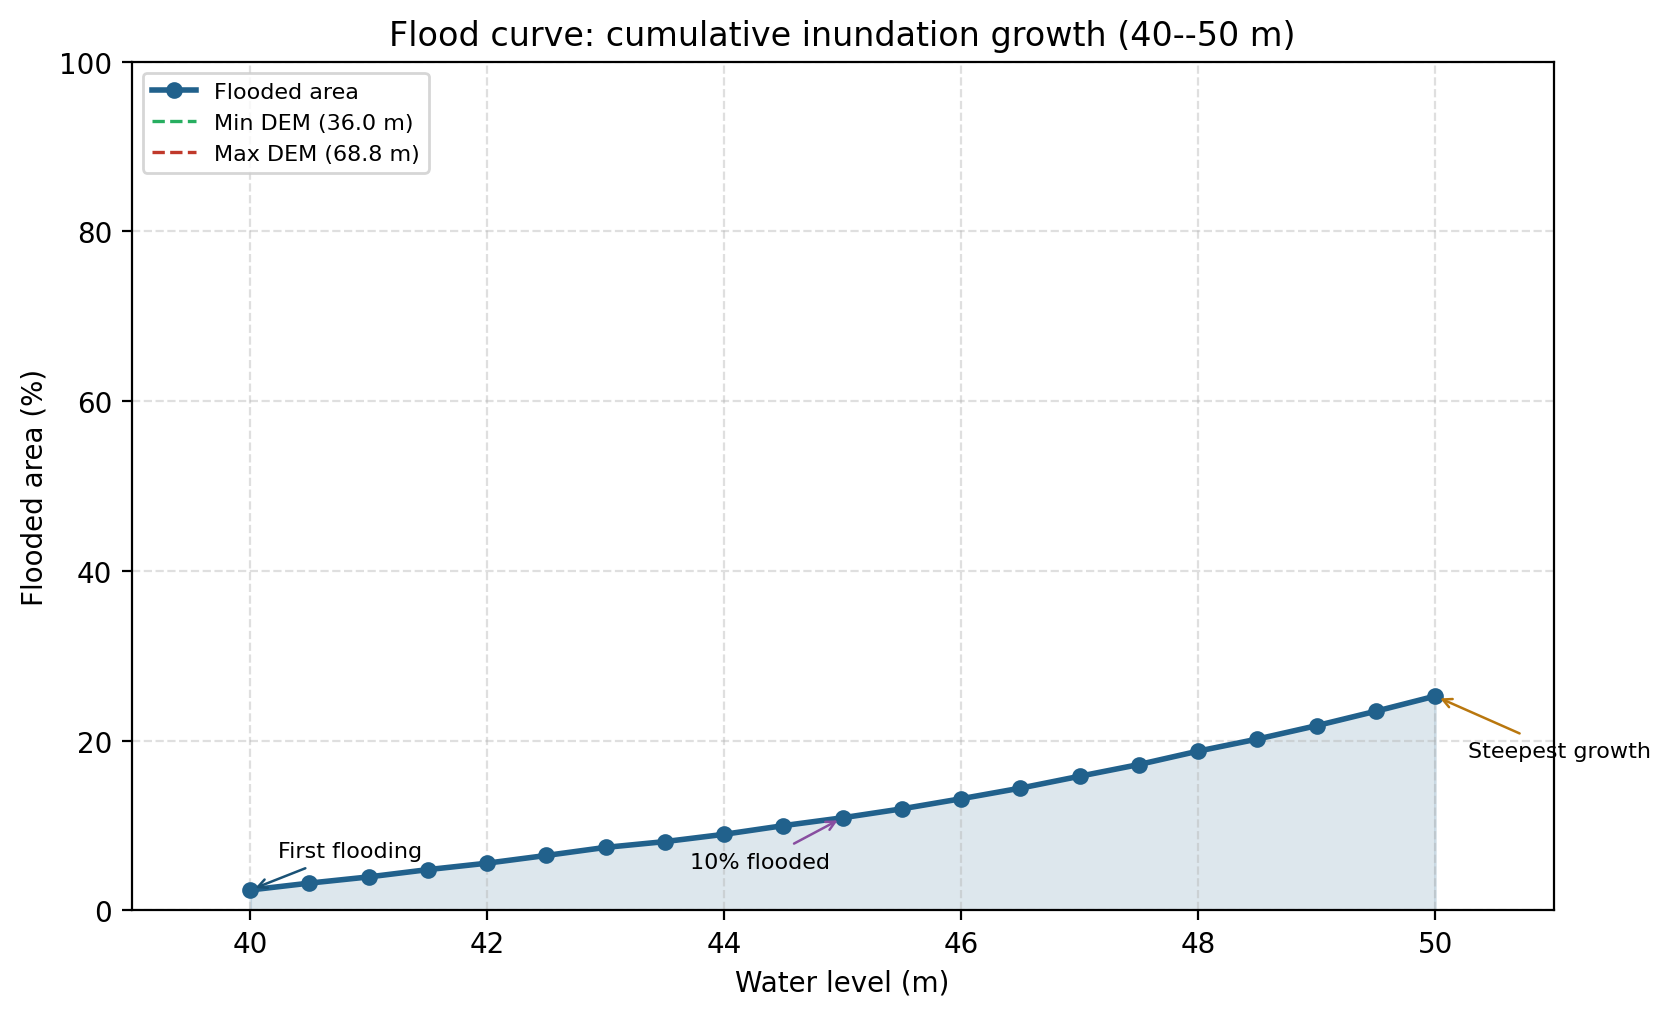
\includegraphics[width=0.88\linewidth,keepaspectratio]{screenshots/flood_curve.png}
  \caption{Flooded area vs water level (annotated growth).}
  \label{fig:curve}
\end{figure}

\begin{figure}[htbp]
  \centering
  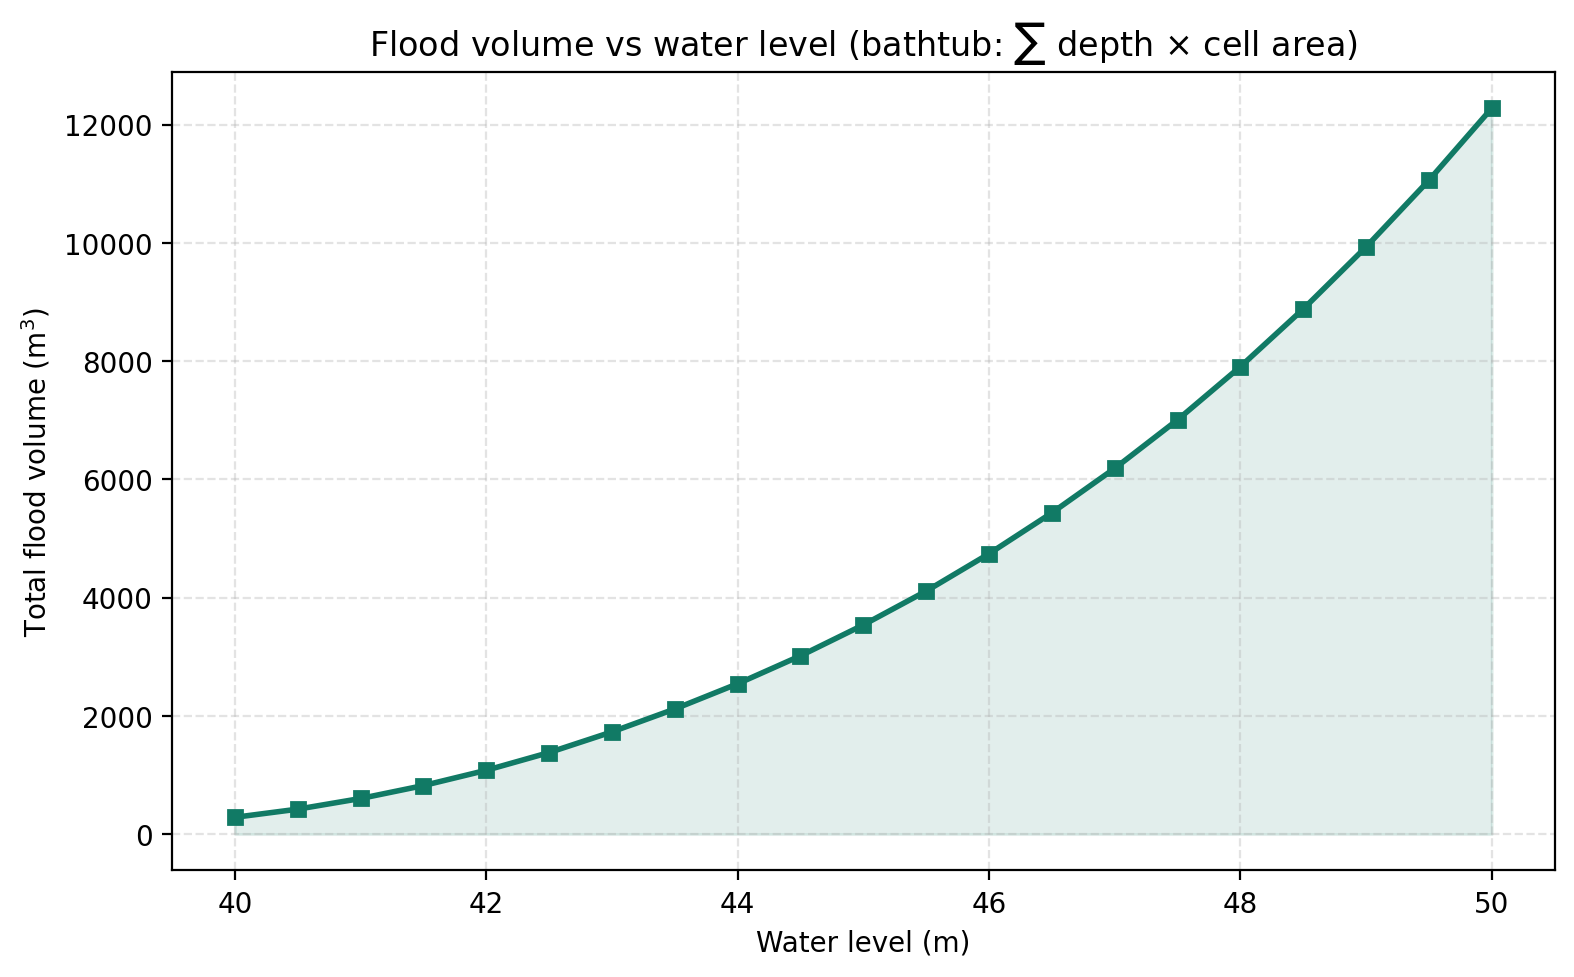
\includegraphics[width=0.88\linewidth,keepaspectratio]{screenshots/flood_volume_curve.png}
  \caption{Total flood volume vs water level (\texttt{flood\_volume\_curve.png}).}
  \label{fig:volcurve}
\end{figure}

%=============================================================================
\section{Part 5: Physical Validation (10\%)}
%=============================================================================

Nine-item PASS/FAIL checklist in \texttt{validate\_flood.py} / \texttt{validation\_report.txt}.

\begin{figure}[htbp]
  \centering
  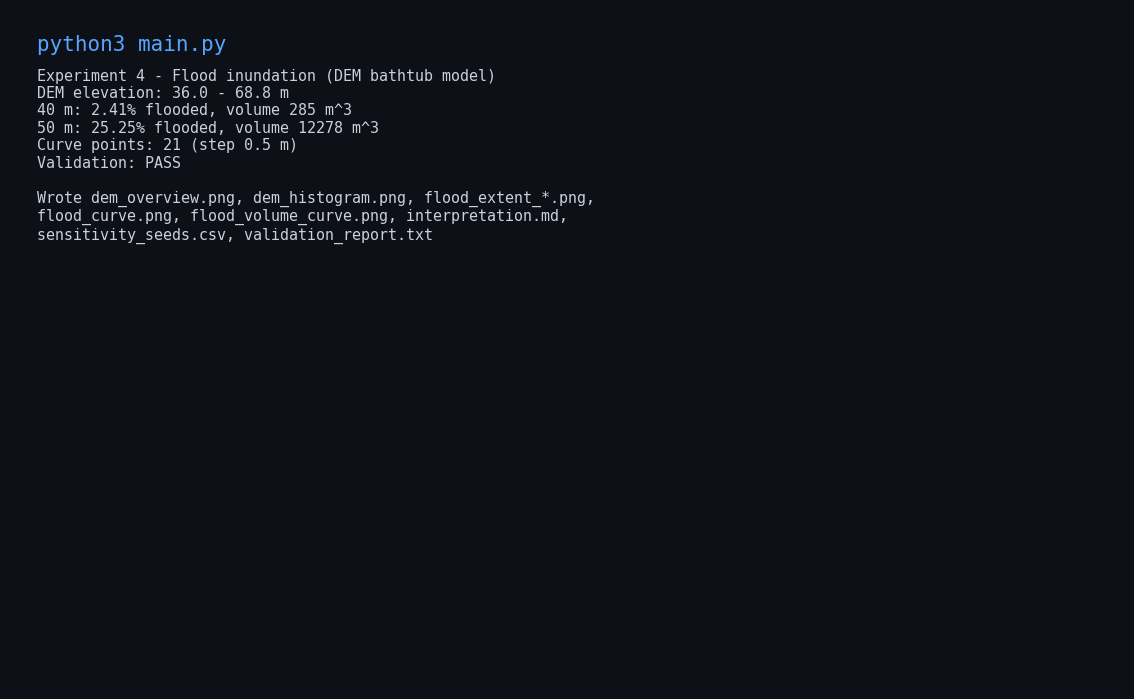
\includegraphics[width=\linewidth]{screenshots/experiment4_main.png}
  \caption{Pipeline run: \texttt{python3 main.py} (DEM load, flood stats at 40/50~m, validation PASS).}
  \label{fig:main}
\end{figure}

\begin{table}[htbp]
  \centering
  \caption{Seed sensitivity: flooded \% at 50~m water level.}
  \label{tab:seed}
  \begin{tabular}{@{}rrr@{}}
    \toprule
    Seed & $z_{\min}$--$z_{\max}$ (m) & Flooded (\%) \\
    \midrule
    42 & 36.0--68.8 & 25.25 \\
    7  & 36.0--69.1 & 25.45 \\
    99 & 35.1--69.4 & 25.04 \\
    \bottomrule
  \end{tabular}
\end{table}

\begin{table}[htbp]
  \centering
  \caption{Runtime benchmark (\texttt{validation\_report.txt}, local machine).}
  \label{tab:bench}
  \begin{tabular}{@{}lr@{}}
    \toprule
    Task & ms \\
    \midrule
    DEM load & 0.25 \\
    Single \texttt{calculate\_flood} & 0.04 \\
    Full curve (21 levels) & 1.78 \\
    \bottomrule
  \end{tabular}
\end{table}

\begin{figure}[htbp]
  \centering
  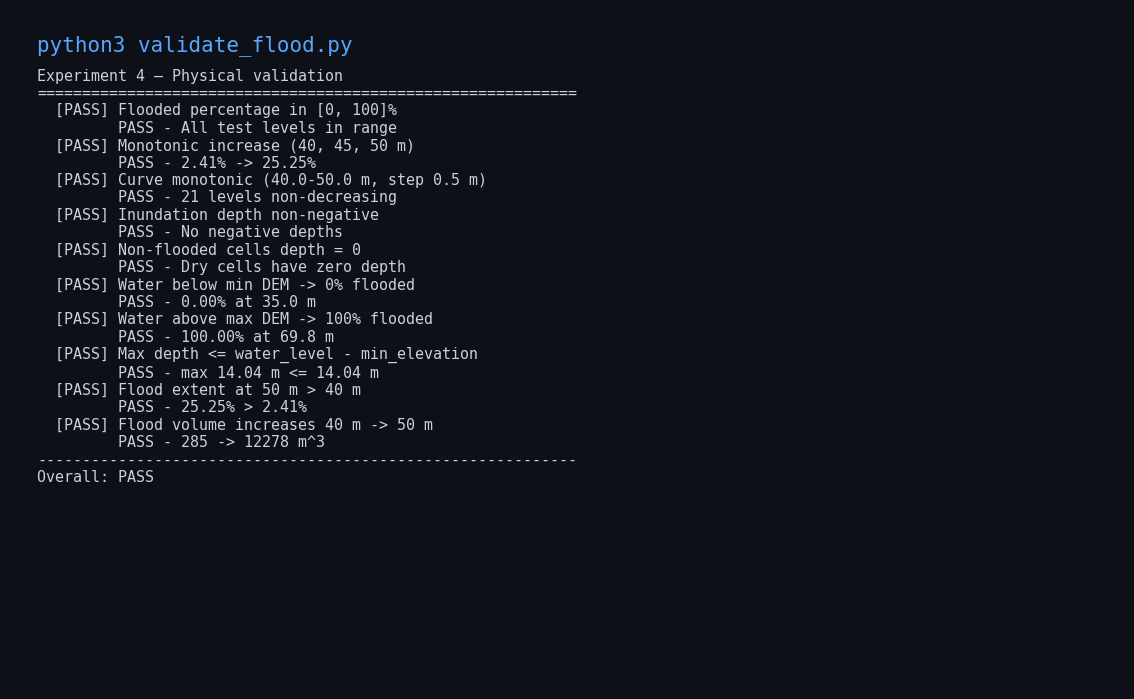
\includegraphics[width=\linewidth]{screenshots/experiment4_validation.png}
  \caption{Validation CLI (\texttt{validate\_flood.py}).}
  \label{fig:validation}
\end{figure}

\begin{figure}[htbp]
  \centering
  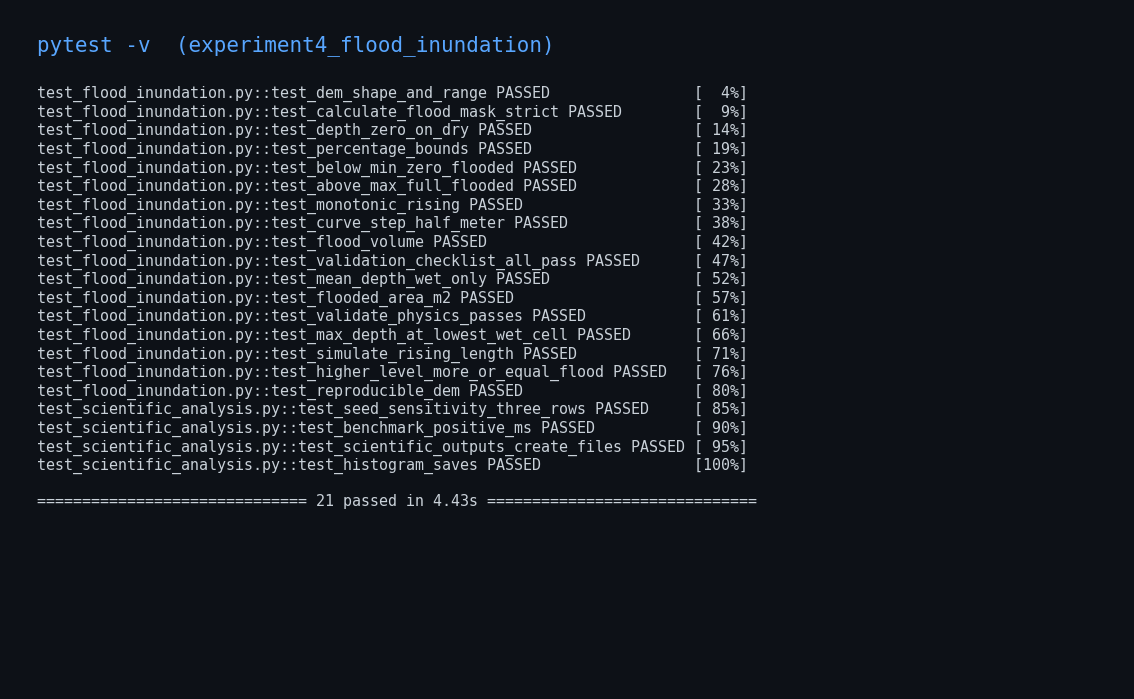
\includegraphics[width=\linewidth]{screenshots/experiment4_pytest.png}
  \caption{21 tests passed (\texttt{pytest -v}).}
  \label{fig:pytest}
\end{figure}

%=============================================================================
\section{Physical Interpretation}
%=============================================================================

\begin{itemize}[noitemsep]
  \item \textbf{Valleys flood first} when $h=40$~m exceeds local lows in the central depression.
  \item \textbf{Accelerated growth} occurs as $h$ crosses the dense part of the elevation histogram (Figure~\ref{fig:hist}).
  \item \textbf{Connected inundation} expands across the valley floor near 48--50~m (Figure~\ref{fig:extent50}).
  \item \textbf{Monotonic area and volume} confirm a consistent flat water surface.
  \item \textbf{Seed sensitivity} shows $\sim$25.0--25.5\% flooded at 50~m for seeds 7/42/99---terrain realization matters modestly on this generator.
\end{itemize}

%=============================================================================
\section{Limitations}
%=============================================================================

\begin{enumerate}[noitemsep]
  \item Flat water surface (no stage gradient).
  \item No hydraulic routing (depressions may not fill without connectivity).
  \item No momentum, infiltration, or evaporation.
  \item No buildings/levees.
\end{enumerate}

Bathtub DEM inundation remains standard for rapid screening and teaching despite these simplifications.

%=============================================================================
\section{Prompt Log (5\%)}
%=============================================================================

Documented in \texttt{prompt\_log.md}. AI-assisted implementation cross-checked per course guidance and \texttt{AGENTS.md}.

\section{AI-Augmented Software Engineering}
\label{sec:ai-eng}

\subsection{Swiss Cheese Model --- layered verification}
\begin{table}[htbp]
  \centering
  \caption{Verification layers (Experiment 4).}
  \label{tab:swiss4}
  \begin{tabular}{@{}ll@{}}
    \toprule
    Layer & Result \\
    \midrule
    AI code review & Strict \texttt{elev $<$ level}; depth = max(0,$\cdot$) \\
    Unit tests & 22 passed \\
    Physical rules & Depth $\ge 0$; monotonic area/volume vs stage \\
    \texttt{validate\_flood.py} & 9/9 PASS \\
    Seed sensitivity & Seeds 7, 42, 99 at 50~m stage \\
    \bottomrule
  \end{tabular}
\end{table}

\subsection{Jagged Frontier --- AI mistake caught}
\textbf{AI output:} Early drafts risked negative depths or non-monotonic flooded area when stage crosses the elevation histogram.

\textbf{Detection:} Physical validation checklist; pytest on curve CSV; visual inspection of 40/50~m maps.

\textbf{Human correction:} Explicit depth convention; \texttt{simulate\_rising\_water()} curve; volume curve; \texttt{interpretation.md}; seed CSV.

\subsection{Tool evaluation (summary)}
Cursor Agent for pipeline and scientific extras; validation CLI is the grader-facing audit layer.

\section{Reproducibility}
%=============================================================================

\begin{verbatim}
pip install -r requirements.txt
python3 main.py
python3 validate_flood.py
pytest -v
python3 generate_report_figures.py
\end{verbatim}

\textbf{Extra outputs:} \texttt{dem\_histogram.png}, \texttt{flood\_volume\_curve.png}, \texttt{sensitivity\_seeds.csv}, \texttt{interpretation.md}.

\section{Conclusion}
Experiment~4 is guide-complete and strengthened with scientific DEM/histogram figures, contour GIS-style maps, annotated and volume curves, sensitivity and timing analysis, interpretation, limitations, 21 pytest cases, and this report.

\appendix
\section{Interpretation excerpt}
\filebox{\texttt{interpretation.md}}{interpretation.md}
\section{Core code}
\filebox{\texttt{flood\_inundation.py} (opening)}{flood_inundation.py}
\section{Prompt log}
\filebox{\texttt{prompt\_log.md}}{prompt_log.md}

\end{document}
